\documentclass[handout]{beamer}
\usepackage{beamerthemesplit}
\usepackage{pgfpages}
\usepackage{verbatim}
\usepackage{amsmath, amssymb, graphics, setspace}
\setbeamercovered{dynamic}
%\pgfpagesuselayout{4 on 1}[a4paper,border shrink=5mm]

\newcommand{\field}[1]{\mathbb{#1}} %requires amsfonts

\usetheme{Antibes}
\usecolortheme{beaver}
\title[S-box Security and Implementations]{Measuring the Cryptographic Security of S-Boxes with Efficient Implementations}

\usepackage{mathptmx}
\usepackage[scaled=.90]{helvet}
\usepackage{courier}
\usepackage[T1]{fontenc}

%\pgfpagesuselayout{4 on 1}[letterpaper,border shrink=5mm]

\institute[RIT]{}
\date{\today}
%\subtitle{}
\author{Christopher A. Wood}
%\institute[]{}
\date{\today}

\begin{document}

%%%%%
%%
%% Resource link: http://www.math-linux.com/spip.php?article77
%%
%%%%

\begin{frame}
	\titlepage
\end{frame}

\begin{frame}
	\frametitle{Agenda}
	\tableofcontents
\end{frame}
\section{Rijndael Review}
\begin{frame}
	\frametitle{Rijndael - The Advanced Encryption Standard}
	\begin{itemize}
		\item Four main operations
		\begin{itemize}
			\item Add round key
			\item Shift rows
			\item Substitute bytes
			\item Mix columns
		\end{itemize}
	\end{itemize}
\end{frame}

% ARK: the actual encryption stage, XOR state matrix with appropriate key block in key schedule
% Implications: How much can we guarantee about the construction of the key schedule? Implies there are good and bad keys that can be used. The algorithm should not have to worry about the usage of a "good" key to be secure.
\begin{frame}
	\frametitle{Add Round Key}
	\begin{center}
      		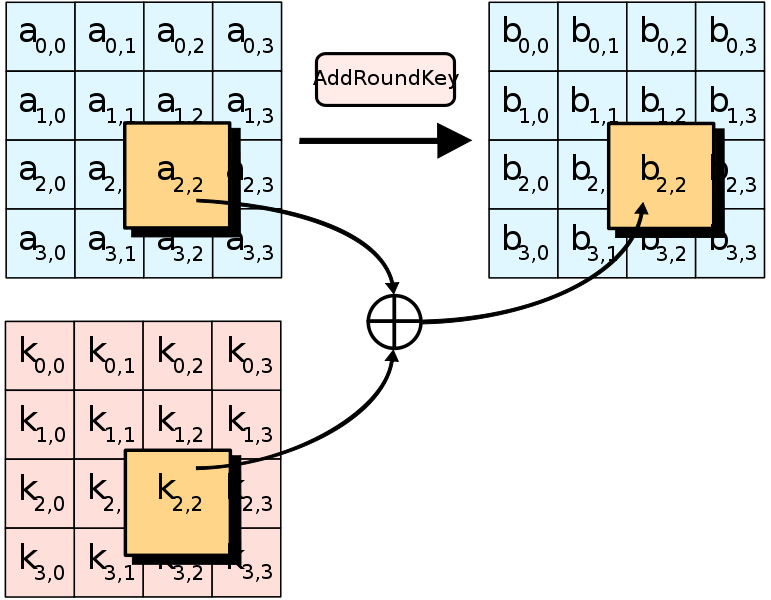
\includegraphics[width=75mm]{images/ark.png}
	\end{center}
\end{frame}

% purpose: just another permutation for diffusion... just rotate the data to avoid linear cryptanalysis. nothing special
\begin{frame}
	\frametitle{Shift Rows}
	\begin{center}
      		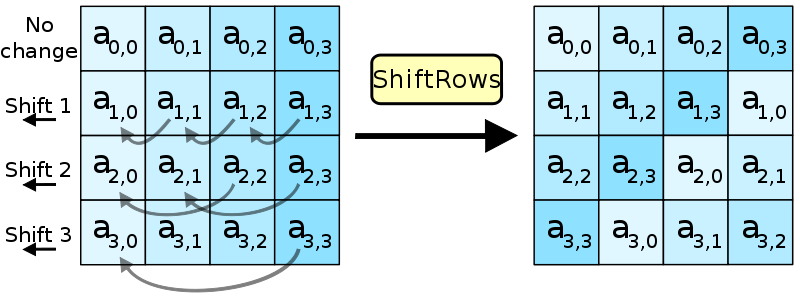
\includegraphics[width=75mm]{images/shift.png}
	\end{center}
\end{frame}

\begin{frame}
	\frametitle{Substitute Bytes} %guarantees about branch number (# of active s-boxes) and the measure of nonlinearity 
	\begin{center}
      		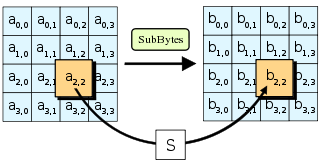
\includegraphics[width=75mm]{images/sub.png}
	\end{center}
\end{frame}

\begin{frame}
	\frametitle{Substitute Bytes}
	This affine transformation can also be represented algebraically as follows
	\begin{eqnarray*}
		b_i' = b_i \oplus b_{(i+4) mod 8} \oplus b_{(i+5) mod 8} \oplus b_{(i+6) mod 8} \oplus b_{(i+7) mod 8} \oplus c_i
	\end{eqnarray*}
	where $i$ is the $i$th bit of the input byte $b$ and $c = \langle 01100011 \rangle$.
\end{frame}

% TODO: mention usage of different MDS matrices
\begin{frame}
	\frametitle{Mix Columns}
	\begin{center}
      		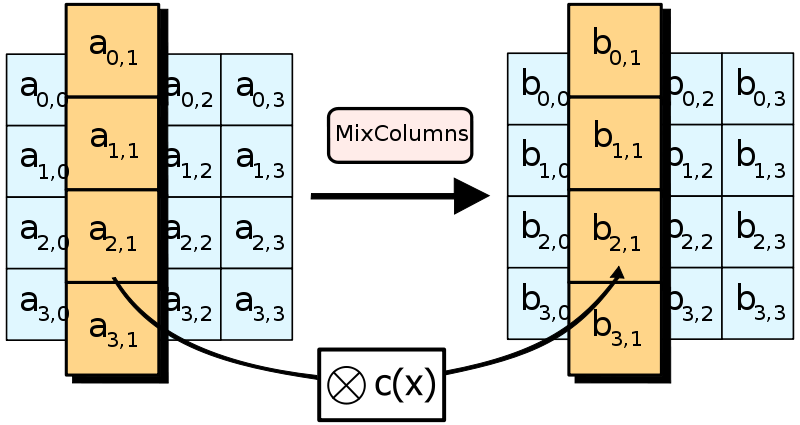
\includegraphics[width=75mm]{images/mix.png}
	\end{center}
\end{frame}

\begin{frame}
	\frametitle{Mix Columns MDS Matrix}
	\begin{center}
      		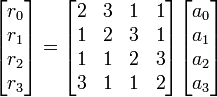
\includegraphics[width=75mm]{images/mix_ops.png} %MDS matrix used for diffusion (why 4x4? other larger wide-pipe designs have been propsed, including 8x8 and 16x16)
	\end{center}
\end{frame}

\section{Design Criteria and Implementation Considerations}
\begin{frame}
	\frametitle{Algorithm security fundamentals}
	\begin{itemize}
		\item Strive for high confusion and diffusion
		\begin{itemize}
			\item \emph{Confusion} - complex relationship between the secret key and ciphertext
			\item \emph{Diffusion} - dissipation of plaintext bits throughout ciphertext bits
		\end{itemize}
	\end{itemize}
\end{frame}

\begin{frame}
	\frametitle{Implementation Considerations}
	\begin{itemize}
		\item Design against common cryptanalysis techniques
		\item Linear transformations
		\begin{itemize}
			\item Linear permutations
			\item Circular shifts
			\item Modular addition
		\end{itemize}
		\item Nonlinear transformations 
		\begin{itemize}
			\item \textbf{S-boxes}
			\item ARX functions
			\item Chaotic recurrence relations
			%\item Number theoretic PRNGs
		\end{itemize}
	\end{itemize}
\end{frame}

\begin{frame}
	\frametitle{S-boxes}
	\begin{itemize}
		\item Bijective functions from $\field{F}_2^n \to \field{F}_2^n$.
		\item Designed for optimal nonlinearity and algebraic complexity.
		\begin{itemize}
			\item Maximize the avalanche property of the S-box for all input/output pairs.
			\item Minimize the differential propagation probability %TODO: make sure this is known
			\item Maximize complexity of the algebraic expression for the S-box in $\field{F}_2^n$
		\end{itemize}
	\end{itemize}
\end{frame}

%TODO: another slide on S-boxes
\begin{frame}
	\frametitle{S-boxes}
	\begin{itemize}
		\item Random and fixed structure (i.e. Rijndael s-box) designs have been proposed based on susceptibility to differential cryptanalysis
		\begin{itemize}
			\item Fixed structure are more beneficial for security analysis and proof purposes
		\end{itemize}
		\item Various construction criteria have been proposed
		\begin{itemize}
			\item Nydberg (91) - \emph{"A perfect nonlinear S-box is a substitution transformation with evenly distributed directional derivatives."}
			\item Dawson and Tavares (91) - static and dynamic criteria supporting claim for high branch numbers and avalanche property
			\item ...
		\end{itemize}
	\end{itemize}
\end{frame}

\section{Measuring S-box Security}
\begin{frame}
	\frametitle{Measuring security}
	\begin{itemize}
		\item Linear behavior
		\begin{itemize}
			\item Exhibit avalanche effect and adherence to Strict Avalanche Criterion (SAC)
		\end{itemize}
		\item Nonlinear behavior
		\begin{itemize}
			\item Branch number
			\item Direct measurement of nonlinear behavior
		\end{itemize}
	\end{itemize}
\end{frame}

\begin{frame}
	\frametitle{Avalanche effect}
A function $f : \field{F}_2^n \to \field{F}_2^n$ exhibits the \emph{avalanche effect} if and only if 
	\begin{eqnarray*}
		\sum_{x \in \field{F}_2^n} \text{wt}(f(x) \oplus f(x \oplus c_{i}^{n})) = n2^{n-1},*
	\end{eqnarray*}
	for all $i (1 \leq i \leq n)$, where $c_{i}^{n} = [0, 0, ..., 1, ..., 0]$ (where a $1$ is in the $n$th position of the vector of cardinality $n$). \\
	%\vspace{0.25cm}
	%This is a significantly stronger sufficient condition for high measures of diffusion.\\
	\vspace{0.25cm}
	*\emph{wt} indicates the Hamming Weight function
\end{frame}

\begin{frame}
	\frametitle{SAC}
	A function $f : \field{F}_2^n \to \field{F}_2^n$ satisfies the \emph{Strict Avalanche Critertion (SAC)} if for all $i (1 \leq i \leq n)$ the following equation holds:
	\begin{eqnarray*}
		\sum_{x \in \field{F}_2^n} f(x) \oplus f(x \oplus c_i^n) = (2^{n-1}, 2^{n-1}, ..., 2^{n-1})
	\end{eqnarray*}
	This simply means that $f(x) \oplus f(x \oplus c_i^n)$ is balanced for every pair of elements in $\field{F}_2^n$ with Hamming distance of $1$. 
\end{frame}

%TODO: include image of avalanche effect

% \begin{frame}
% 	\frametitle{Branch number}
% 	The \emph{branch number} of an $n \times n$-bit S-Box is
% 	\begin{eqnarray*}
% 		BN = \text{min}_{a, b\not=a}(\text{wt}(a \oplus b) + \text{wt}(S(a) \oplus S(b))),
% 	\end{eqnarray*}
% 	where $a, b \in \field{F}_2^n$.
% \end{frame}

%TODO: include another slide about branch number (with different definition?)

\begin{frame}
	\frametitle{S-box specific nonlinear measurements}
	The nonlinearity of an $n$-bit S-Box from $\field{F}_2^n \to \field{F}_2^n$ can be measured by
	\begin{eqnarray*}
		P_S = \text{max}_{0 \not= a, b}|\{x \in \field{F}_2^n : S(x + a) - S(x) = b\}|
	\end{eqnarray*}
	where $a, b \in \field{F}_2^n$.
\end{frame}

%http://fse2012.inria.fr/SLIDES/kaisa.pdf
\begin{frame}
	\frametitle{Bent Functions}
	The correlation between a Boolean function $f : \field{F}_2^n \to \field{F}_2$ and a linear function $x \mapsto u \cdot x$ is defined as
	\begin{eqnarray*}
	c_f(u) = \frac{1}{2^n}(|\{x \in \field{F}_2^n : f(x) = u \cdot x\}| - |\{x \in \field{F}_2^n : f(x) \not= u \cdot x\}|)
	\end{eqnarray*}
	A Boolean function is thus called \emph{bent} if
	\begin{eqnarray*}
		|c_f(u)| = 2^{\frac{-n}{2}},
	\end{eqnarray*}
	for all $u \in \field{F}_2^n$. Note that $n$ must be even in order for $f$ to be bent.
\end{frame}

\begin{frame}
	\frametitle{Vector Bent Functions}
	\begin{itemize}
		\item Perfect nonlinearity of Boolean functions strongly correlates to cryptographic strength
		\item Nydberg's "perfect nonlinear functions" - vectorial Boolean functions
	\end{itemize}
	A vector function $f : \field{F}_2^n \to \field{F}_2^m$ is said to be \emph{bent} if
	\begin{itemize}
		\item $w \cdot f_i$ is bent for all $w \not= 0, 1 \leq i \leq m$.
		\item $f$ is perfectly nonlinear ($f(x + \alpha) = f(x)$ is uniformly distributed as $x$ varies, for all fixed $\alpha \in \field{F}_2^n - \{0\}$).
	\end{itemize}
\end{frame}

\begin{frame}
	\frametitle{APN S-boxes}
	A function $f : \field{F}_2^n \to \field{F}_2^n$ is said to be \emph{almost perfect nonlinear} (APN) if
	\begin{eqnarray*}
		|\{x : f(x + \alpha) + f(x) = \beta\}| \leq 2,
	\end{eqnarray*}
	for all fixed $\alpha \in \field{F}_2^n - \{0\}$. Some examples include:
	\begin{itemize}
		\item $f : \field{F}_2^n \to \field{F}_2^n, f(x) = x^3$
		\item $f : \field{F}_2^n \to \field{F}_2^n, f(x) = x^{2^{k} + 1}$ (i.e. any odd power exponent)
	\end{itemize}
\end{frame}

\begin{frame}
	\frametitle{Differentially $\delta$-Uniform S-box functions}
	A function $f : \field{F}_2^n \to \field{F}_2^n$ is said to be \emph{differentially $\delta$-uniform} if
	\begin{eqnarray*}
		|\{x : f(x + \alpha) + f(x) = \beta\}| \leq \delta,
	\end{eqnarray*}
	Small values for $\delta$ are desirable - indicates higher degree of nonlinearity.
\end{frame}

\subsection{Some Other Nonlinear Transformations}
\begin{frame}
	\frametitle{ARX functions}
	\begin{itemize}
		\item Nonlinear functions consisting of a combination of addition, bitwise rotation, and bitwise XOR operations
		\item Analysis of differential propagation is difficult
		\begin{itemize}
			\item Differential properties of sub-operations need to be considered (adp$^{\oplus}$, xdp$^{+}$)
		\end{itemize}
		\item Most susceptible to rotational cryptanalysis
		\begin{itemize}
			\item Threefish was attacked using a combination of rotational cryptanalysis with a rebound attack (Khovratovich et al, 2010) - led to adjustment of Threefish rotation constants %rotational crypt can essentially be thought of as DC but treating pairs of words as (unrotated, rotated) and looking at p(rotate(x+y) == rotate(X) + rotate(y))
		\end{itemize}
	\end{itemize}
\end{frame}

%TODO: another slide and MORE details on ARX functions - see Threefish paper?
%\begin{frame}
%	\frametitle{ARX functions}
%	\begin{itemize}
%		\item 
%	\end{itemize}
%\end{frame}

\begin{frame}
	\frametitle{Chaotic recurrence relations}
	\begin{itemize}
		\item Chaotic systems are defined by:
		\begin{itemize}
			\item Sensitivity to initial conditions 
			\item Topologically mixing (i.e. covers entire state space)
			\item Dense (and long) periodic orbits 
		\end{itemize}
		\item Some recurrence relations exhibit "chaotic" behavior (e.g. the Logistic Map)
	\end{itemize}
	\begin{eqnarray*}
		x_{n+1} = rx_{n}(1 - (x_{n}))
		\label{logisticmap}
	\end{eqnarray*}
\end{frame}

\begin{frame}
	\frametitle{Chaos in the Logistic Map}
	\begin{center}
      		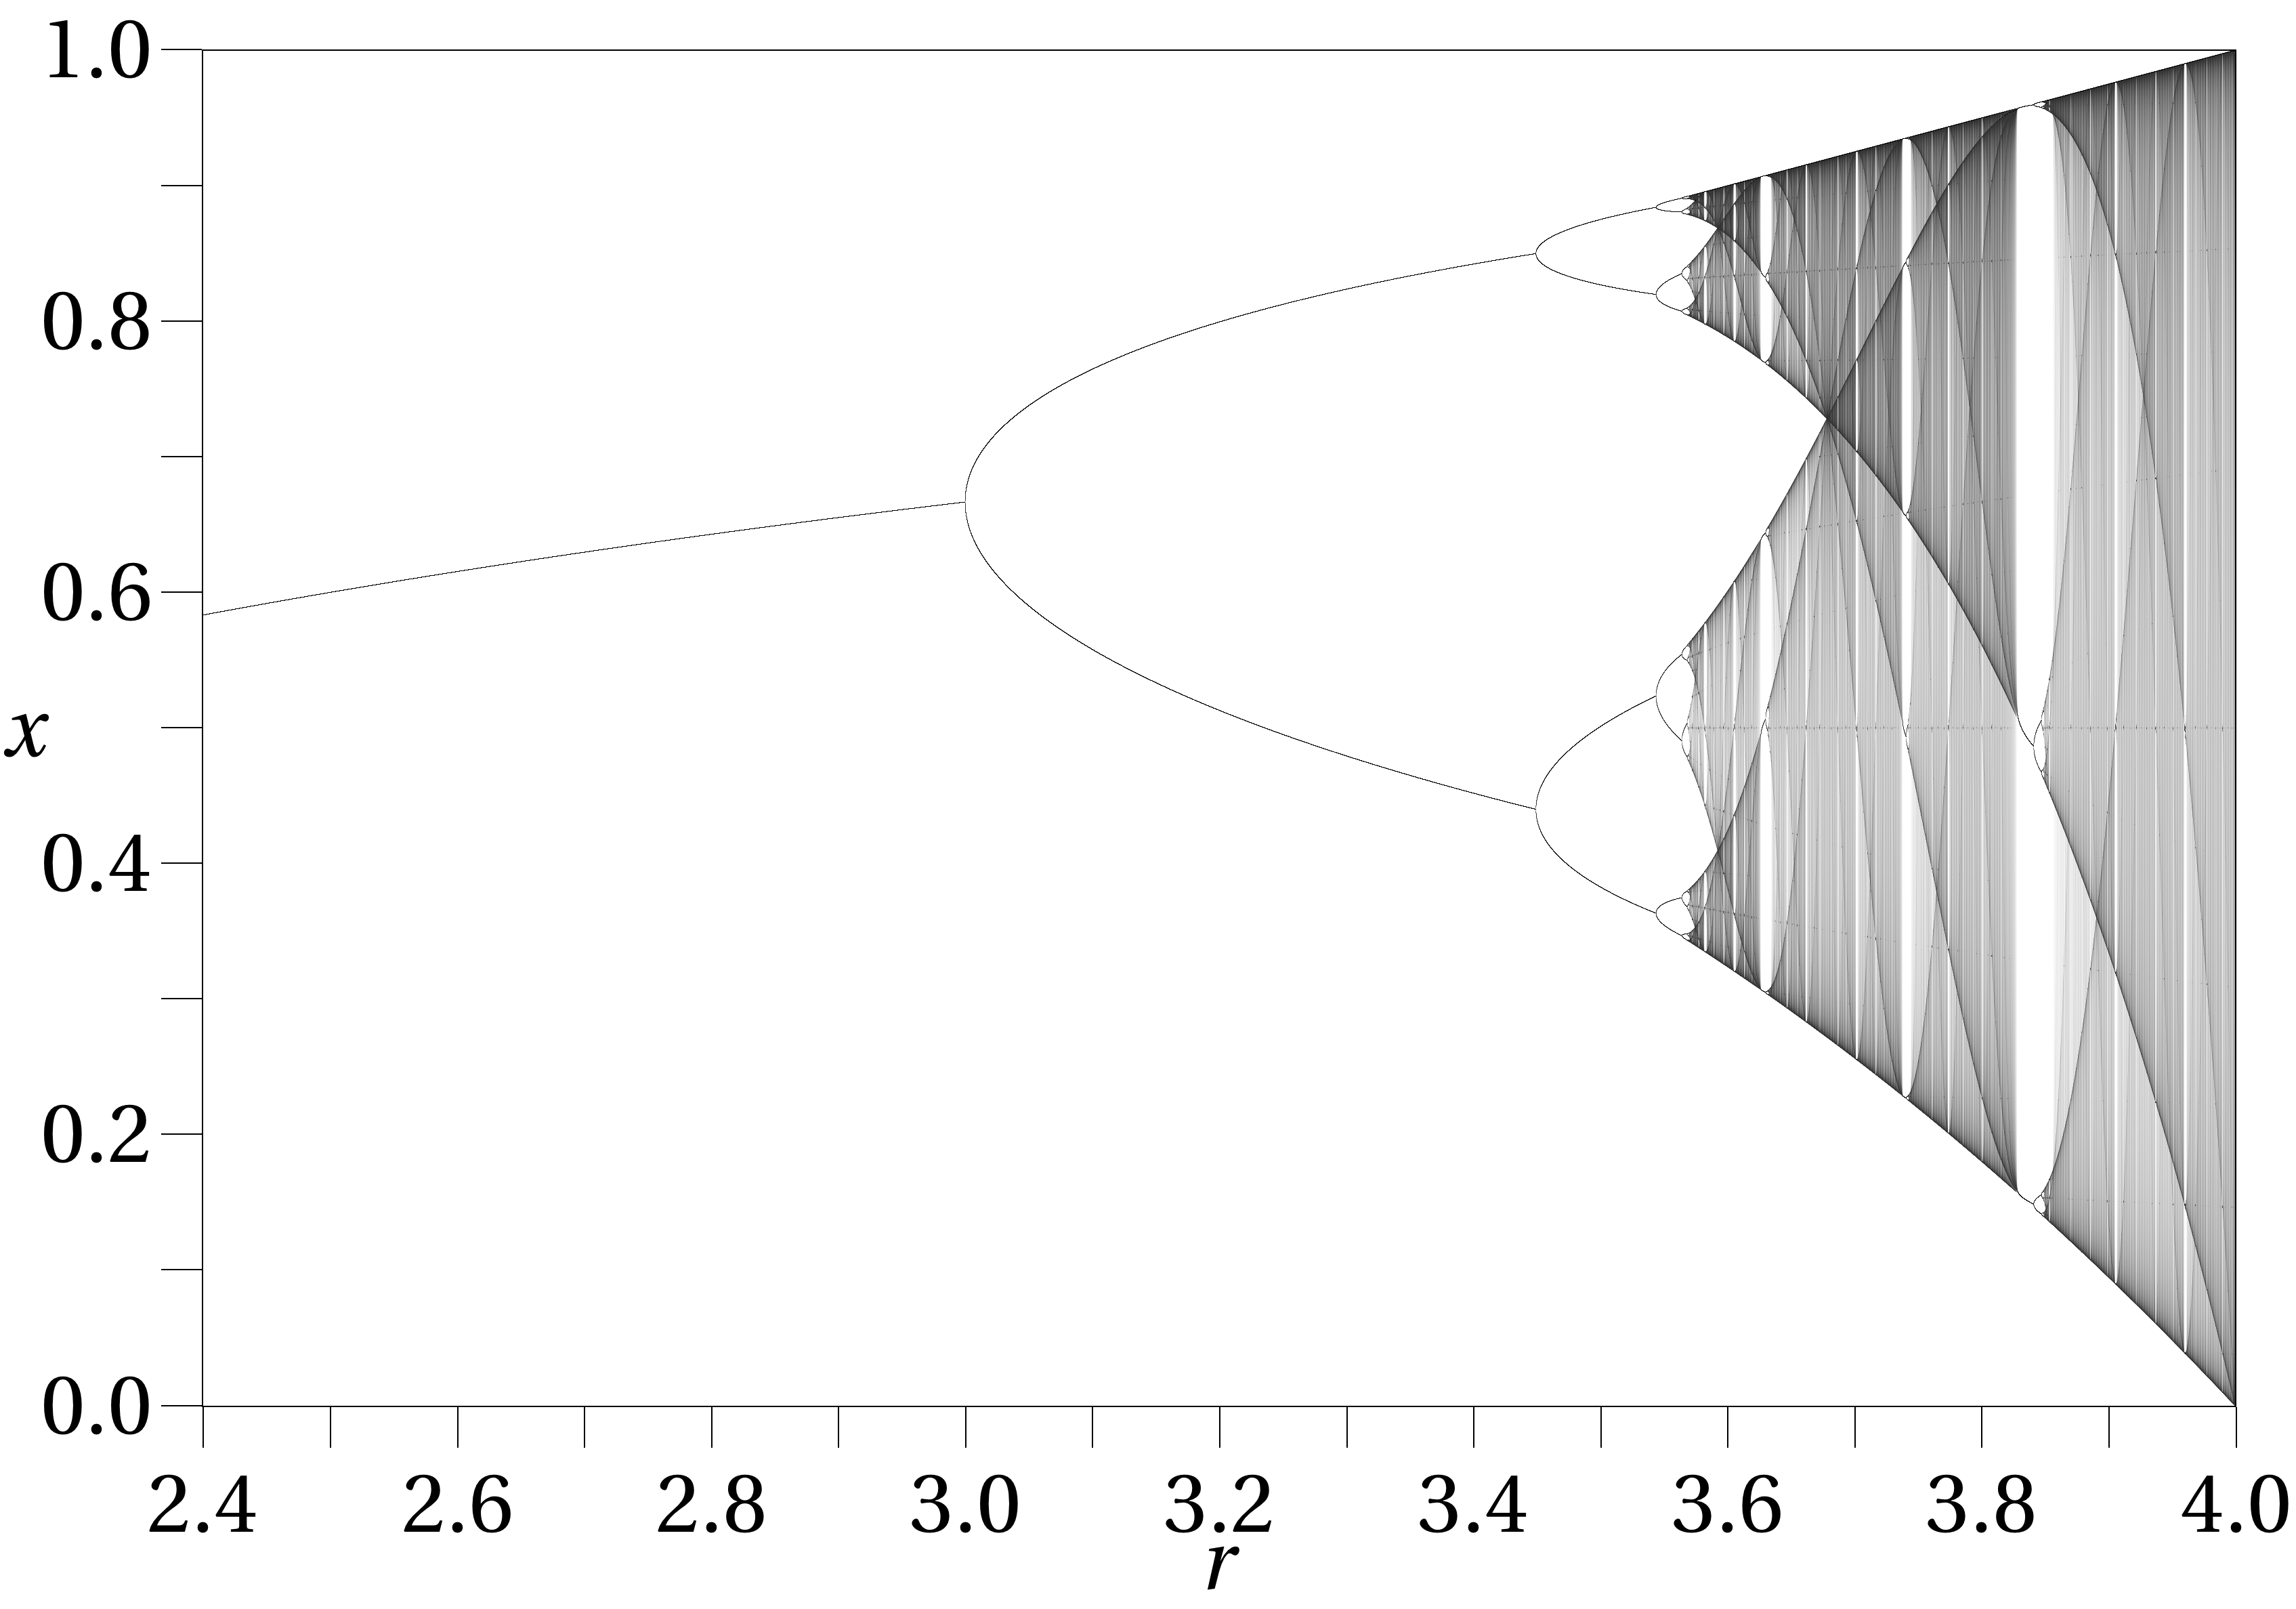
\includegraphics[width=90mm]{images/logistic_bifurcation.png}
	\end{center}
\end{frame}

\section{Implementation Strategies}
\begin{frame}
\frametitle{Changing Gears}
Now that we've measure the security and chosen the right S-box, we must now implement it!
\end{frame}

\subsection{Composite Fields}
\begin{frame}
	\frametitle{Composite Fields}
	A \emph{composite field} is a pair 
	\begin{align*}
	& \{GF(2^n), Q(y) = y^n + \sum_{i=0}^{n-1}q_iy^i, q_i \in GF(2)\} \\
	& \{GF((2^n)^m), P(x) = x^m + \sum_{i=0}^{m-1}p_ix^i, p_i \in GF(2^n)\},
	\end{align*}
	where $GF(2^n)$ is constructed from $GF(2)$ by $Q(y)$, and $GF((2^n)^m)$ is
	constructed from $GF(2^n)$ by $P(x)$. Also, $GF((2^n)^m)$ is a degree $m$ extension
	of $GF(2^n)$.
\end{frame}

\subsection{Composite Fields for Rijndael}
\begin{frame}
\frametitle{Rijndael S-box}
The S-box in Rijndael is defined as follows:
\begin{align*}
F(x) = Ax^{-1} \oplus b,
\end{align*}
where $x, b \in GF(2^8)$.

\medskip

Computing the inverse of $x$ with combinational logic in hardware is \emph{very} expensive. What can we do?
\end{frame}

\begin{frame}
	\frametitle{Computing the Inverse with Composite Fields}
	Every element in a field $GF(2^{nm})$ can be represented by a polynomial with coefficients from $GF(2^n)$ using 
	an irreducible polynomial of the form $x^2 + Ax + B$ (we assume $m = 2$). Thus, if $\alpha \in GF(2^{nm})$, and $\alpha = bx + c$, where $b,c \in GF(2^n)$, then:
	\begin{align*}
	\alpha^{-1} = (bx + c)^{-1} = b(b^2B + bcA + c^2)^{-1} + (c + bA)(b^2B + bcA + c^2)^{-1}
	\end{align*}
	\pause
	Now we compute the inverse over $GF(2^n)$, leading to less required hardware resources.
\end{frame}

\begin{frame}
\frametitle{Composite Field Representations}
Research has systematically examined all composite field extensions for $GF(2^8)$, seeking to minimize the area.
\begin{align*}
GF(2^4) \to GF((2^4)^2) \\
GF(2^2) \to GF((2^2)^4) \\
GF(2^2) \to- GF((2^2)^2) \to GF(((2^2)^2)^2)
\end{align*}
A systematic evaluation must check all tower field extensions \textbf{and} all irreducible polynomials.
\end{frame}

\begin{frame}
	\frametitle{8-Bit S-Boxes}
	Satoh tower field design - $GF(((2^2)^2)^2)$
	\begin{center}
	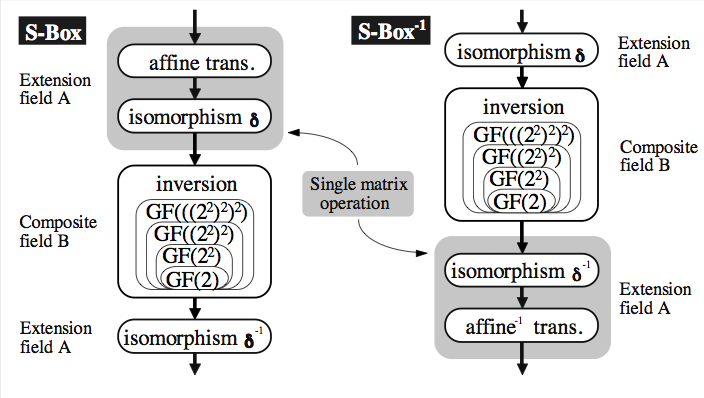
\includegraphics[scale=.35]{./images/tower8bit.png}
	\end{center}
\end{frame}

\begin{frame}
	\frametitle{16-Bit S-Boxes}
	Proposed design - $GF((((2^2)^2)^2)^2)$
	\begin{center}
	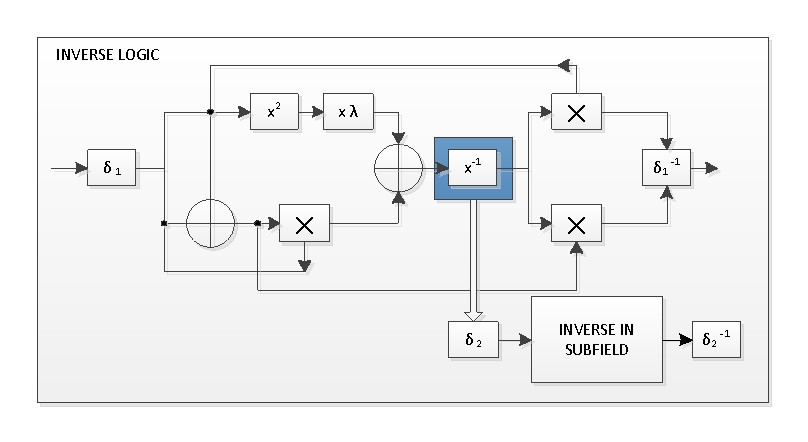
\includegraphics[scale=0.65]{./images/composite_field_inverter.pdf}
	\end{center}
	\textbf{Question:} How deep should this recursion go? What yields the minimal hardware area?
\end{frame}

\subsection{Tower Field Isomorphic Functions}
\begin{frame}
\frametitle{Tower Field Isomorphic Functions}
The isomorphic functions are constructed as follows (assume we're constructing a function for mapping $GF(2^{nm}) \to GF((2^n)^m)$):
\begin{itemize}
	\item Find two generators $\alpha$ and $\beta$ ($\alpha \in GF(2^{nm})$ and $\beta \in GF((2^n)^m)$), where $\alpha$ and $\beta$ are roots of the same primitive irreducible polynomial. 
	\item Map $\alpha^k \to \beta^k$ for $1 \leq k \leq 2^{nm}$ (mapping basis elements of $GF(2^{nm}) \to GF((2^n)^m)$). If the mapping doesn't hold group homomorphism, find the next generator $\beta$ and repeat.
\end{itemize}
\end{frame}

\begin{frame}
	\frametitle{Isomorphic Function Generation - Primitive Irreducible Polynomials}
	The isomorphic mappings are constructed as follows (assume we're constructing a function for mapping $GF(2^{nm}) \to GF((2^n)^m)$):
	\begin{itemize}
		\item Find two generators $\alpha$ and $\beta$ ($\alpha \in GF(2^{nm})$ and $\beta \in GF((2^n)^m)$), where $\alpha$ and $\beta$ are roots of two respective primitive polynomials.
		\item Map $\alpha^k$ to $\beta^k$ for $1 \leq k \leq 2^{nm}$.
		\item Multiplication and addition homomorphism is guaranteed. 
		\begin{itemize}
			\item $\alpha^i \times \alpha^j = \alpha^{i + j} = \beta^{i + j} = \beta^i \times \beta^j$
			\item $\alpha^t = \alpha^i + \alpha^j \to \beta^t = \beta^j + \beta^j$
		\end{itemize}
	\end{itemize}
\end{frame}

\begin{frame}
	\frametitle{Isomorphic Function Generation - Exhaustive Searches}
	\begin{itemize}
		\item Find two generators $\alpha$ and $\beta$ ($\alpha \in GF(2^{nm})$ and $\beta \in GF((2^n)^m)$).
		\item Map $\alpha^k$ to $\beta^k$ for $1 \leq k \leq 2^{nm}$ (multiplication homomorphism holds)
		\item For all $0 \leq i \leq 2^{nm} - 1$ check to see if $\alpha^i + 1 \to \beta^i + 1$.
		\item Multiplication and addition homomorphism is now guaranteed.
		\begin{itemize}
			\item $\alpha^i \times \alpha^j = \alpha^{i + j} = \beta^{i + j} = \beta^i \times \beta^j$
			\item $\alpha^t = \alpha^i + \alpha^j = \alpha^i \times (1 + \alpha^{j - i}) \to \beta^t = \beta^i \times (1 + \beta^{j - i}) = \beta^i + \beta^j$
		\end{itemize}
	\end{itemize}
\end{frame}

\begin{frame}
	\frametitle{Matrix Transformation \textbf{T}}
	The matrix \textbf{T} can be generated with the following algorithm.
	\begin{itemize}
		\item Let $\beta$ be a generator of $GF((2^n)^m)$ such that $\alpha^i \in GF(2^{nm})$ is mapped to $\beta^i$ for all $0 \leq i \leq 2^{nm} - 1$ ($\alpha$ forms a basis of $GF((2^n)^m)$).
		\item Compute $\alpha^0, \alpha^1, \alpha^2,\dots,\alpha^{nm - 1}$.
		\item Define the columns of \textbf{T} as the transpose of each $nm$-dimensional bit vector of these powers:
\begin{align*}
		\textbf{T} =  \left[ \begin{array}{cccc}
(\alpha^{nm - 1})^T & \dots & (\alpha^{1})^T (\alpha^{0})^T \end{array} \right]
\end{align*}
	\end{itemize}
\end{frame}

\begin{frame}
\frametitle{An Example}
\begin{itemize}
	\item $\alpha = x$ and $\beta = xy$
	\item $(x^7 + x^6 + x^5 + x^2 + x + 1) \to [(x^3 + x^2 + x + 1)y + (x^3 + x^2 + 1)]$
	\item $\textbf{T} =  \left[ \begin{array}{cccc}
(xy^{nm - 1})^T & \dots & (xy^{1})^T (xy^{0})^T \end{array} \right]$
\end{itemize}

\begin{align*}
\left( \begin{array}{cccccccc}
0 & 0 & 1 & 0 & 0 & 0 & 1 & 0 \\
0 & 1 & 1 & 0 & 0 & 1 & 0 & 0 \\
0 & 0 & 0 & 1 & 1 & 0 & 1 & 0 \\
1 & 0 & 0 & 1 & 0 & 0 & 0 & 0 \\
1 & 1 & 1 & 0 & 1 & 0 & 0 & 0 \\
0 & 1 & 1 & 1 & 0 & 1 & 0 & 0 \\
1 & 0 & 1 & 0 & 1 & 0 & 0 & 0 \\
0 & 1 & 0 & 1 & 0 & 1 & 0 & 1 \\ \end{array} \right) \left( \begin{array}{c}
1 \\
1 \\
1 \\ 
0 \\
0 \\ 
1 \\
1 \\ 
1 \end{array} \right) = \left( \begin{array}{c}
1 \\
1 \\
1 \\ 
1 \\
1 \\ 
1 \\
0 \\ 
1 \end{array} \right)
\end{align*}
\end{frame}

\begin{frame}
\frametitle{Another Example}
\begin{itemize}
	\item $\alpha = x$ and $\beta = xy$ (same homomorphic mapping)
	\item $(x^6) \to [(x^2)y + (x^3 + x^2 + 1)]$
	\item $\textbf{T} =  \left[ \begin{array}{cccc}
(xy^{nm - 1})^T & \dots & (xy^{1})^T (xy^{0})^T \end{array} \right]$
\end{itemize}

\begin{align*}
\left( \begin{array}{cccccccc}
0 & 0 & 1 & 0 & 0 & 0 & 1 & 0 \\
0 & 1 & 1 & 0 & 0 & 1 & 0 & 0 \\
0 & 0 & 0 & 1 & 1 & 0 & 1 & 0 \\
1 & 0 & 0 & 1 & 0 & 0 & 0 & 0 \\
1 & 1 & 1 & 0 & 1 & 0 & 0 & 0 \\
0 & 1 & 1 & 1 & 0 & 1 & 0 & 0 \\
1 & 0 & 1 & 0 & 1 & 0 & 0 & 0 \\
0 & 1 & 0 & 1 & 0 & 1 & 0 & 1 \\ \end{array} \right) \left( \begin{array}{c}
0 \\
1 \\
0 \\ 
0 \\
0 \\ 
0 \\
0 \\ 
0 \end{array} \right) = \left( \begin{array}{c}
0 \\
1 \\
0 \\ 
0 \\
1 \\ 
1 \\
0 \\ 
1 \end{array} \right)
\end{align*}
\end{frame}

\section{16-bit S-boxes}
\begin{frame}
	\frametitle{Different Tower Field Decompositions for 16-bit S-boxes}
	\begin{align*}
	(1)\text{ } GF(2^{16}) & \to GF((2^8)^2) \\ 
	(2)\text{ } GF(2^{16}) & \to GF((2^4)^4) \\ 
	(3)\text{ } GF(2^{16}) & \to GF((2^2)^8) \\
	\end{align*}
	We need only study these decompositions - optimal tower-field decompositions for smaller fields are in the literature.
\end{frame}

\begin{frame}
	\frametitle{Multiplicative Inverse Calculations}
	The derivation gets messy very quick...
	\begin{align*}
	(b*x^3+c*x^2+d*x+e)*(f*x^3+g*x^2+h*x+i)\text{=}\\
	k*(x^4+A*x^3+B*x^2+C*x+D)+1
	\end{align*}
	
	\begin{align*}
	f \to \frac{1}{x^3 \left(e+d x+c x^2+b x^3\right)}\left(1-e i+D k-e h x-d i x+C k x\right) \\ \left(-e g x^2-d h x^2-c i x^2+B k x^2-d g x^3-c
h x^3-b i x^3+A k x^3-c g x^4\right) \\ \left(-b h x^4+k x^4-b g x^5\right)
	\end{align*}
	\begin{center}
		Are there easier ways to calculate the inverse?
	\end{center}
\end{frame}

\begin{frame}
	\frametitle{Finding Capable Polynomials}
	\begin{itemize}
		\item Primitive polynomials always work for the mapping
		\begin{itemize}
			\item Let $\alpha$ be a primitive root of the field $F_2[x]/P(x)$ and $P(\alpha) = 0$
			\item $P(x)$ is therefore a \emph{primitive polynomial}
			\item Powers $\alpha$ (which are linearly independent) can be used to form a standard basis
		\end{itemize} 
		\item Exhaustive generate all primitive polynomials up to degree $16$ (there exists $a_p(n) = \frac{\phi(p^n - 1)}{n}$ polynomials for degree $n$)
		\item Choose the one that has the lowest transformation and multiplication/inverse costs
	\end{itemize}
\end{frame}

\begin{frame}
	\frametitle{Finding Capable Polynomials (cont'd)}
	\begin{table}
		\begin{tabular}{|l|l|}
		\hline
		Degree & Primitive Polynomials  \\ \hline
		1 & $x + 1$  \\ 
		2 & $x^2 + x + 1$  \\
		3 & $x^3 + x + 1$, $x^3 + x^2 + 1$  \\
		4 & $x^4 + x^3 + 1$, $x^4 + x + 1$  \\
		5 & $x^5 + x^2 + 1$, $x^5 + x^3 + x^2 + x + 1$, $x^5 + x^4 + x^3 + x + 1$ \\
		\hline
		\end{tabular}
	\end{table}
	For $n = 16$, we have $a_2(16) = \frac{\phi(2^16 - 1)}{n} = 2048$ different primitive polynomials.
\end{frame}

\begin{frame}
	\frametitle{Choosing the Right Transform}
	\begin{itemize}
		\item Let \textbf{T}$^*$ be the optimal transformation matrix in the set of transformations $\mathcal{T}$.
		\item The ``cost'' of transforms is the number of 1s in the matrix \textbf{T}$^*$. 
		\item The ``cost'' of the inverse is dependent on the polynomial selection.
	\end{itemize}
	\begin{align*}
	T^* = \min_{T_i \in \mathcal{T}}\{C(transform) + C(inverse) + C(invTransform)\}
	\end{align*}
	\begin{itemize}
		\item Examine all primitive polynomials for $P(x)$, $Q(x)$, $R(x)$
		\item Generate all possible composite field transformations
		\item Pick the one with least cost
	\end{itemize}
\end{frame}

\begin{frame}
	\frametitle{Exhaustively Searching All S-boxes}
	\begin{itemize}
		\item Loop over invertible binary matrices and all constants for affine transformation
		\item For each valid mapping, measure the cryptographic strength using the Boolean function
		analysis software
		\item Pick the one with the best properties
	\end{itemize}
\end{frame}

\begin{frame}
	\frametitle{An Interesting Case}
	\begin{itemize}
		\item Nyberg's Power Mapping: $F(x) = x^{2^{k} + 1}$
		\item These functions are $2$-differentially uniform with a $\mathcal{N}_l$ equal to precisely $2^{n-1} - 2^{\frac{n-1}{2}}$.
		\begin{itemize}
			\item That's better than the inverse mapping $F(x) = x^{-1}$
		\end{itemize}
		\item In a normal basis, this reduces to squaring (which is free) and multiplications
		\item For hardware, does this yield a more efficient \textbf{and} more secure mapping for $16$-bit S-boxes?
	\end{itemize}
\end{frame}

%\begin{frame}
%	\frametitle{Walsh transformation measurement}
%	\begin{itemize}
%		\item TODO
%	\end{itemize}
%\end{frame}

\begin{comment}
\begin{frame}
	\frametitle{Provable Security for S-boxes}
	\textbf{Theorem: } (KN Theorem) It is assumed that in a DES-like cipher with $f :  \field{F}_2^m \to  \field{F}_2^n$ (the substitution function) the keys are independent and uniformly random. Then, the probability of an s-round differential, $s \geq 4$, is less than or equal to $p_{max}^2$, where $p_{max}$ is defined in terms of the nonlinearity of the S-box as follows:
	\begin{eqnarray*}
		p_{max} \leq max_{b} max_{a \not= 0} Pr[f(Y + a) + f(a) = b],
	\end{eqnarray*}
	where $a, b \in \field{F}_2^n$.
	% How valid is the random key distribution assumption?
	% Y is some other element in the field... just go back to nonlinearity example
\end{frame}

\begin{frame}
	\frametitle{Similar Nonlinear Functions}
	\begin{itemize}
		\item Bent functions
		\item Vector bent functions
		\item APN S-boxes
		\item Differentially $\delta$-Uniform S-box functions
		\item ...
	\end{itemize}
\end{frame}
\end{comment}

\end{document}
